\section{Artificial Neural Network Overview}
This section will give a short overview of the applied network pattern and the learning algorithm used for training of the network. The overview will be based on the more detailed explanation in Section~\ref{sec:annSection}.

\subsection{Structure}
Feed-forward will be the preferred architecture for predicting the electricity prices and wind power productions in this thesis. It is the most common structure and data flows from the input to the output layer through the hidden layers in between. The input layer will consist of all the the influential factors of wind power or electricity price and the output will be the predicted price or wind power. Figure~\ref{fig:overviewAnn} illustrates the concept well.

\begin{figure}[!ht]
\centering
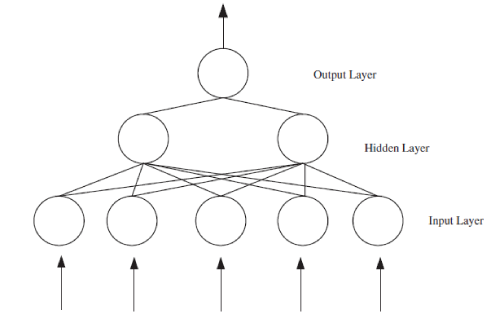
\includegraphics[width=0.8\linewidth]{billeder/ANN.png}
\caption{A simple neural network with 3 layers. \cite{stockForecasting}}
\label{fig:overviewAnn}
\end{figure}

\subsection{Learning}
Training of the network network will be done with the Resilient Back-propagation algorithm. It is faster than standard back propagation \cite{8,15} and is often used with the feedforward architecture which we use here \cite{14,17}. In short i